\section{Phương pháp chia đổi (The Bisection Method)}

Một trong những kỹ thuật cơ bản nhất để giải phương trình phi tuyến $f(x) = 0$ là 
\textit{phương pháp chia đôi} (Bisection Method). 
Ý tưởng dựa trên \textit{Định lý Giá trị Trung gian}: 
nếu $f$ liên tục trên khoảng $[a,b]$ và $f(a)f(b) < 0$, 
thì tồn tại ít nhất một nghiệm $p \in (a,b)$ sao cho $f(p) = 0$.  

Phương pháp tiến hành như sau:  
bắt đầu với khoảng $[a,b]$, ta tính trung điểm
\[
p = \frac{a+b}{2}.
\]
Nếu $f(p) = 0$, nghiệm đã được tìm thấy. 
Ngược lại, tùy thuộc vào dấu của $f(p)$, ta chọn nửa khoảng chứa nghiệm:  
\[
[a,p] \quad \text{nếu } f(a)f(p)<0, 
\qquad \text{hoặc} \qquad
[p,b] \quad \text{nếu } f(p)f(b)<0.
\]
Quy trình này được lặp lại cho đến khi khoảng có độ dài nhỏ hơn sai số cho phép $\text{TOL}$.

\begin{figure}[h!]
\centering
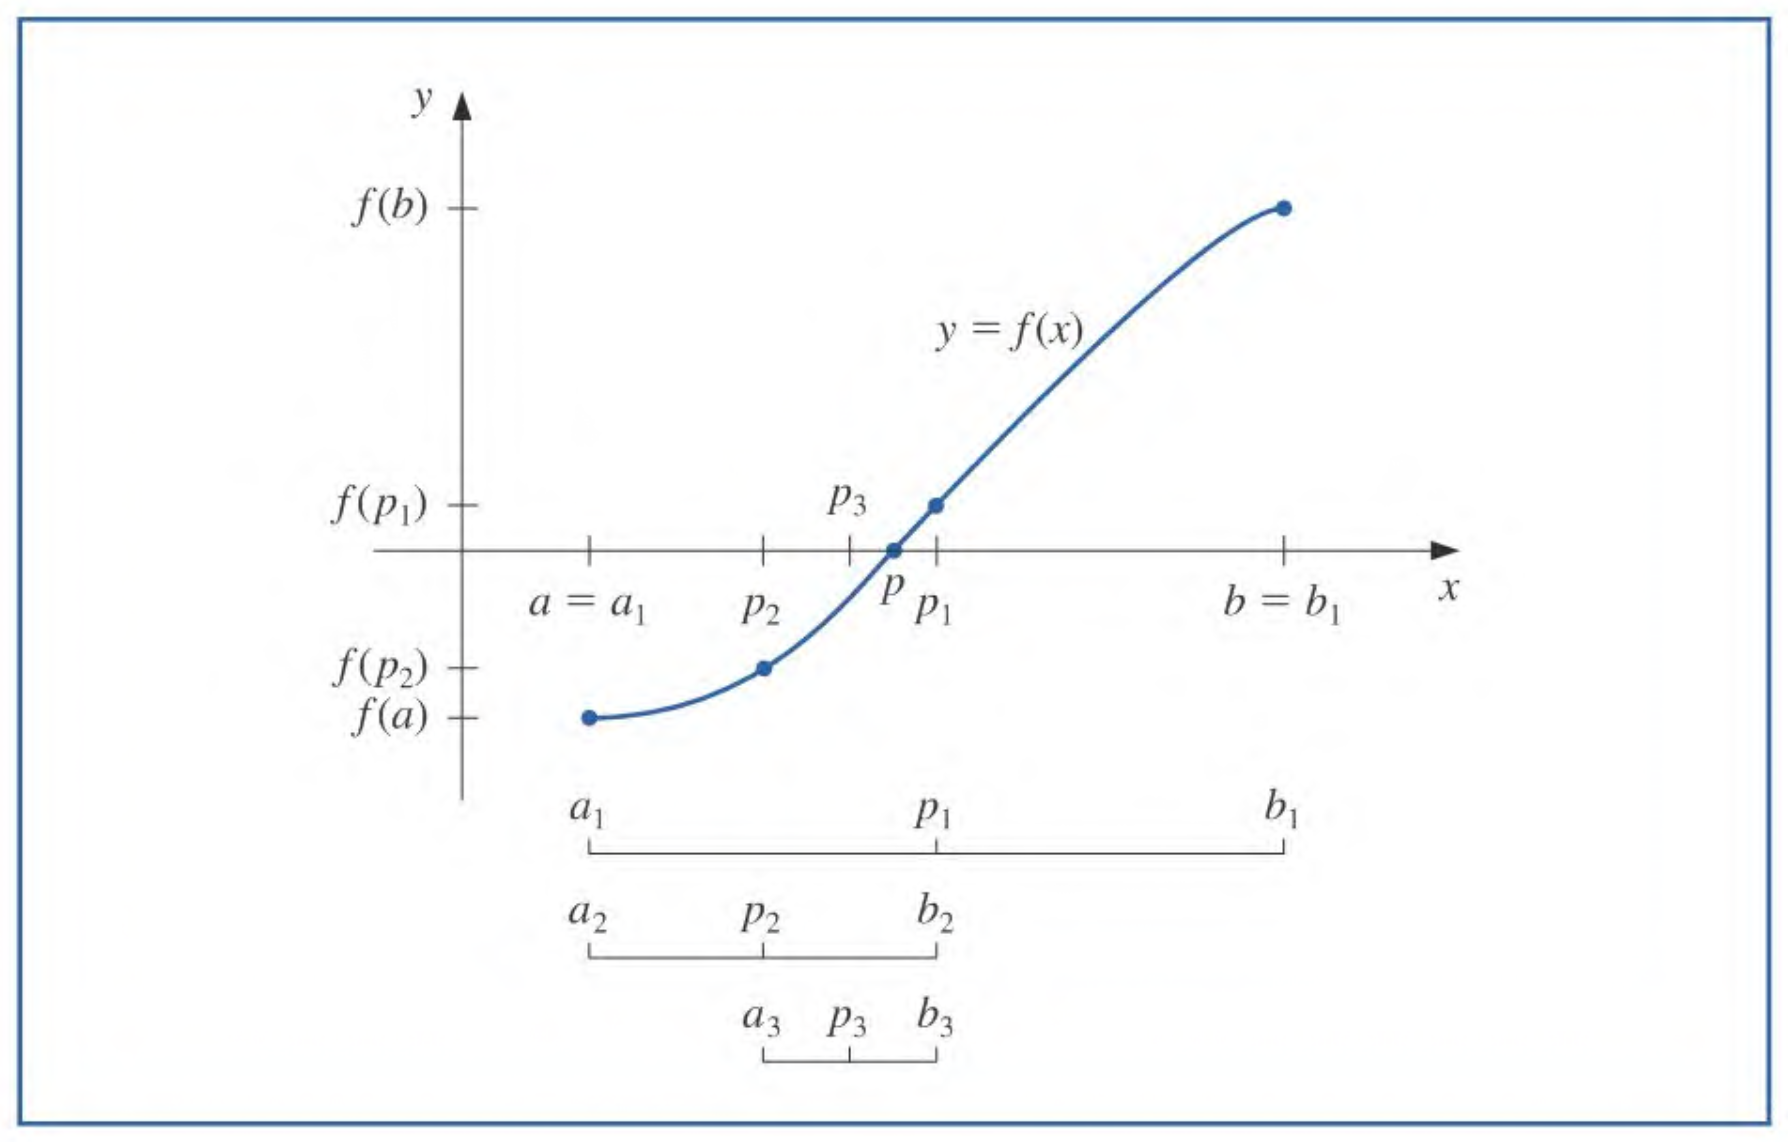
\includegraphics[width=0.7\textwidth]{assets/figure2.1.png}
\caption{Minh họa phương pháp chia đôi (Figure 2.1).}
\label{fig:bisection-fig21}
\end{figure}

\subsection*{\textbf{Thuật toán (Bisection Method)}}

\begin{enumerate}
    \item Chọn $a, b$ sao cho $f(a)f(b)<0$, cùng số lần lặp tối đa $N$ và sai số $\text{TOL}$.
    \item Với $i=1,2,\dots,N$:
    \begin{enumerate}
        \item Tính $p = \tfrac{a+b}{2}$.
        \item Nếu $|f(p)| < \text{TOL}$ hoặc $\tfrac{b-a}{2} < \text{TOL}$, kết thúc và nhận $p$ là nghiệm gần đúng.
        \item Nếu $f(a)f(p)>0$, đặt $a=p$; ngược lại, đặt $b=p$.
    \end{enumerate}
\end{enumerate}

Nếu sau $N$ bước mà chưa đạt điều kiện dừng, thuật toán được xem là thất bại.

\subsection*{\textbf{Ví dụ 1: Phương pháp chia đôi}}

Chứng minh rằng phương trình
\[
f(x) = x^3 + 4x^2 - 10 = 0
\]
có nghiệm trong khoảng $[1,2]$, và sử dụng phương pháp chia đôi để tìm nghiệm xấp xỉ với độ chính xác ít nhất $10^{-4}$.

\textbf{Lời giải.}  
Vì $f(1) = -5 < 0$ và $f(2) = 14 > 0$, nên theo Định lý Giá trị Trung gian, tồn tại ít nhất một nghiệm trong $[1,2]$.  

Ở lần lặp đầu tiên, $p_1 = 1.5$ và $f(1.5) = 2.375 > 0$, do đó nghiệm thuộc khoảng $[1,1.5]$.  
Tiếp tục chia đôi, $p_2 = 1.25$ với $f(1.25) = -1.7969 < 0$, nên nghiệm nằm trong $[1.25,1.5]$.  
Lặp lại quá trình này, ta thu được các giá trị trong Bảng~1.1.

\begin{center}
\captionof{table}{Các bước của phương pháp chia đôi cho $f(x) = x^3 + 4x^2 - 10$}
\begin{tabular}{|c|c|c|c|c|}
\hline
$n$ & $a_n$ & $b_n$ & $p_n$ & $f(p_n)$ \\
\hline
1  & 1.0000 & 2.0000 & 1.5000 & 2.3750 \\
2  & 1.0000 & 1.5000 & 1.2500 & -1.7969 \\
3  & 1.2500 & 1.5000 & 1.3750 & 0.1621 \\
4  & 1.2500 & 1.3750 & 1.3125 & -0.8484 \\
5  & 1.3125 & 1.3750 & 1.3438 & -0.3510 \\
6  & 1.3438 & 1.3750 & 1.3594 & -0.0964 \\
7  & 1.3594 & 1.3750 & 1.3672 & 0.0324 \\
8  & 1.3594 & 1.3672 & 1.3633 & -0.0322 \\
9  & 1.3633 & 1.3672 & 1.3652 & 0.000072 \\
10 & 1.3633 & 1.3652 & 1.3643 & -0.01605 \\
11 & 1.3643 & 1.3652 & 1.3647 & -0.00799 \\
12 & 1.3647 & 1.3652 & 1.3650 & -0.00396 \\
13 & 1.3650 & 1.3652 & 1.3651 & -0.00194 \\
\hline
\end{tabular}
\end{center}

Sau 13 lần lặp, ta được nghiệm xấp xỉ
\[
p_{13} = 1.365112305,
\]
với sai số
\[
|p - p_{13}| < |p_{14} - p_{13}| = |1.365234375 - 1.365112305| = 0.00012207,
\]
nên đảm bảo chính xác ít nhất $10^{-4}$.  
Giá trị đúng của nghiệm (chính xác đến 9 chữ số thập phân) là
\[
p = 1.365230013.
\]

\subsection*{\textbf{Định lý}}

Giả sử $f$ là hàm liên tục trên đoạn $[a,b]$ và thỏa $f(a)f(b) < 0$.  
Khi áp dụng phương pháp chia đôi, ta thu được một dãy $\{p_n\}_{n=1}^\infty$ hội tụ về nghiệm $p$ của $f(x)=0$.  
Hơn nữa, sai số tại bước lặp thứ $n$ được ước lượng bởi
\[
|p_n - p| < \frac{b-a}{2^n}, \quad n \geq 1.
\]

\textbf{Hệ quả.}  
Dãy $\{p_n\}$ hội tụ về $p$ với tốc độ $O(2^{-n})$, tức là
\[
p_n = p + O(2^{-n}).
\]

\subsection*{\textbf{Ví dụ 2: Ước lượng số lần lặp}}

Xác định số lần lặp cần thiết để giải phương trình
\[
f(x) = x^3 + 4x^2 - 10 = 0
\]
với độ chính xác $10^{-3}$, sử dụng $a_1 = 1$ và $b_1 = 2$.

\textbf{Lời giải.}  
Theo Định lý, sai số sau $N$ lần lặp thỏa
\[
|p_N - p| \leq \frac{b-a}{2^N}.
\]
Với $a=1, b=2$, ta có
\[
|p_N - p| \leq \frac{1}{2^N}.
\]

Để đạt độ chính xác $10^{-3}$, cần
\[
\frac{1}{2^N} \leq 10^{-3}
\quad \Rightarrow \quad
N \geq \frac{3}{\log_{10} 2} \approx 9.96.
\]

Vậy cần ít nhất $N=10$ lần lặp để đảm bảo nghiệm gần đúng nằm trong sai số $10^{-3}$.


